\section{Graphs}

In Königsberg in Prussia, there is an island connected
with bridges to the banks of a river.

\begin{figure}
    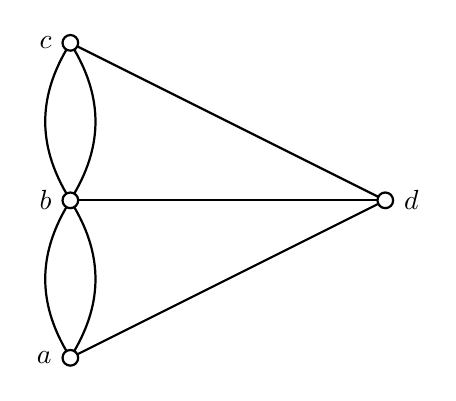
\begin{tikzpicture}[thick, main/.style = {draw, circle}]
        \node[main,scale=0.6, label=left:$a$] (a) at (0,0) {};
        \node[main,scale=0.6, label=left:$b$] (b) at (0,2) {};
        \node[main,scale=0.6, label=left:$c$] (c) at (0,4) {};
        \node[main,scale=0.6, label=right:$d$] (d) at (4,2) {};

        \draw (a) -- (d);
        \draw (b) -- (d);
        \draw (c) -- (d);
        \draw (a) to [out=120,in=240,looseness=1] (b);
        \draw (a) to [out=60,in=300,looseness=1] (b);

        \draw (b) to [out=120,in=240,looseness=1] (c);
        \draw (b) to [out=60,in=300,looseness=1] (c);

    \end{tikzpicture}
    \caption{The Seven Bridges of Königsberg}
\end{figure}

It was asked whether anyone could arrange a route in
such a way that he could cross each bridge once and
only once. Euler modelled the island and banks as
\emph{nodes}. Formally, this question asks if there is a cyclic
path that uses each edge once and only once. It turns out
there is provided the graph is connected and all nodes have
even degree.

Some terminology:

\begin{itemize}
    \item \textbf{Node}: Also known as points or vertices. Fundemental
          building block of a graph.
    \item \textbf{Edge}: Connects two nodes, or a node to itself.
    \item \textbf{Walk}: A sequence of vertices and edges, where the edges connect the adjacent vertices in the sequence.
    \item \textbf{Tour}: A walk with no repeated edges.
    \item \textbf{Path}: A walk with no repeated vertices. A \emph{simple} path has no repeated nodes.
    \item \textbf{Adjacent}: Said of two nodes connected by an undirected edge,
          or of the node to which a directed edges enters and the node of the edge's origin.
    \item \textbf{Degree}: Number of edges going out from a node. In a directed graph,
          there are both in and out degrees.
          \marginnote{Edges that go out from and enter the same node add two degrees to that node.}
    \item \textbf{Cycle}: A path from a node to itself. If there is a cycle in a
          graph, it is a cyclic graph. Else it is acyclic.
    \item \textbf{Connected}: An undirected graph is connected if every node can be reached
          from every other node. For a directed graph, the same property is called strongly connected.
\end{itemize}

Some notation: an undirected graph $G(V,E)$ consists of a set of nodes $V$
and edges $E$. Perhaps $V = {A, B, C}$ and $E = {(A,B), (A,A), (A, C)}$.
A directed graph $G<V, E>$ might have the same vertices, but edges
$E = {<A,B>, <A,A>, <A, C>}$ indicating that one may only travel from $A$
to other nodes.

There are two kinds of graph, \emph{directed} and \emph{undirected}.
In an undirected graph like the one shown previously, an edge can
go both ways. In a directed graph one can travel only one way along an
edge, represented by an arrow like in figure \ref{fig:directedgraph}

\begin{figure}
    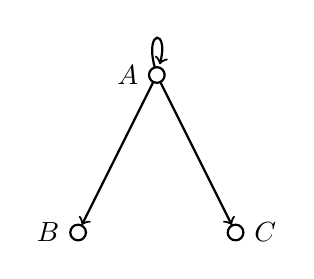
\begin{tikzpicture}[thick, main/.style = {draw, circle}]
        \node[main,scale=0.6, label=left:$A$] (a) at (0,2) {};
        \node[main,scale=0.6, label=left:$B$] (b) at (-1,0) {};
        \node[main,scale=0.6, label=right:$C$] (c) at (1,0) {};

        \draw[->] (a) -- (b);
        \path[->] (a) edge [loop above] ();
        \draw[->] (a) -- (c);

    \end{tikzpicture}
    \caption{Example of a Directed Graph}
    \label{fig:directedgraph}
\end{figure}

A \emph{weighted} graph has weights assocted with each directed edge. The weight
could represent probability of moving from one node to another, travel times, distances,
etc.

\subsection{Adjacency Matrix}

An \emph{adjacency matrix} is a way to represent a graph using a
2D array. For a graph with $n$ nodes, the adjacency matrix is an
$n \times n$ matrix where:

\begin{itemize}
    \item Each row and column corresponds to a node.
    \item The value at position $(i, j)$ is:
          \begin{itemize}
              \item $1$ (or the weight of the edge) if there
                    is an edge from node $i$ to node $j$.
              \item $0$ if there is no edge between node $i$ and node $j$.
          \end{itemize}
\end{itemize}

For an undirected graph, the adjacency matrix is symmetric,
meaning $A[i][j] = A[j][i]$. For a directed graph, the matrix
is not necessarily symmetric.

\textbf{Example:} Consider the directed graph in Figure
\ref{fig:directedgraph}. Its adjacency matrix is:

\[
    \begin{bmatrix}
        1 & 1 & 1 \\
        0 & 0 & 0 \\
        0 & 0 & 0
    \end{bmatrix}
\]

Here:
\begin{itemize}
    \item The value $1$ at $(1,1)$ represents the self-loop on $A$.
    \item The value $1$ at $(1,2)$ and $(1,3)$ represents edges from $A$ to $B$ and $A$ to $C$.
    \item All other entries are $0$ because there are no other edges.
\end{itemize}

\subsection{Linked List}

A \emph{linked list} representation of a graph uses an array of linked lists. Each node in the array represents a vertex, and the linked list at each index contains the neighbors of that vertex.

\textbf{Example:} Consider the directed graph in Figure \ref{fig:directedgraph}. Its linked list representation is:

\begin{itemize}
    \item $A \to A \to B \to C$
    \item $B \to \emptyset$
    \item $C \to \emptyset$
\end{itemize}

Here:
\begin{itemize}
    \item The first list represents the neighbors of $A$:
          a self-loop to $A$, and edges to $B$ and $C$.
    \item The second and third lists are empty because $B$ and
          $C$ have no outgoing edges.
\end{itemize}

The original nodes $A$, $B$, and $C$ can be stored in another
linked list, array, or whatever data structure is convenient.

\subsection{Graph Searching}

There are tow methods to traverse a graph.

\begin{itemize}
    \item Breadth First Search:
          A \emph{breadth first search} (BFS) visits all edges of distance $k$ from
          the source before visiting edges of distance $k+1$ from the source.
          Think of the waves rippling from a pebble thrown into a pond.
    \item Depth First Search:
          A \emph{depth first search} (DFS) visits one edge to the next node, then one edge from
          that node to the next. It goes downa  given path as far as possible
          before returning.
\end{itemize}

Breadth first lends itself to iteration, while depth first lends itself
to recursion.